%\documentclass[tikz, border=5pt]{standalone}
\begin{document}
	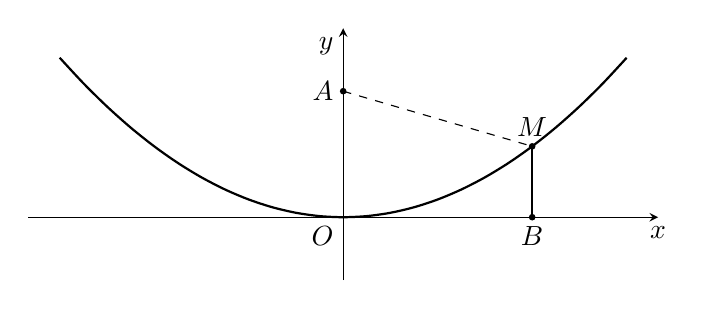
\begin{tikzpicture}[>=stealth, scale=0.8]
		% 1. 绘制坐标轴
		\draw[->] (-5,0) -- (5,0) node[below] {$x$};  % x轴
		\draw[->] (0,-1) -- (0,3) node[below left] {$y$};% y轴
		\node at (0,0) [below left] {$O$};            % 原点标记
		
		% 2. 绘制抛物线 \(8y = x^2\)(即 \(y = \frac{x^2}{8}\))
		\draw[thick, domain=-4.5:4.5, smooth, variable=\x] 
		plot ({\x}, {\x*\x/8});
		
		% 3. 定义并标记关键点
		\coordinate (A) at (0, 2);  % 点A(y轴上)
		\coordinate (B) at (3, 0);    % 点B(x轴上)
		\coordinate (M) at (3, 9/8);  % 点M(抛物线上,\(x=2\) 时 \(y=\frac{2^2}{8}=0.5\))
		
		% 4. 绘制辅助线
		\draw[dashed] (A) -- (M);  % 虚线连接A和M
		\draw[thick] (M) -- (B);   % 实线连接M和B(垂直x轴)
		
		% 5. 标记点(实心小圆+标签)
		\fill (A) circle (1.5pt) node[left] {$A$};
		\fill (B) circle (1.5pt) node[below] {$B$};
		\fill (M) circle (1.5pt) node[above] {$M$};
	\end{tikzpicture}
\end{document}
